\documentclass{standalone}
\usepackage{pgfplots}
\usepgfplotslibrary{groupplots}
\pgfplotsset{compat=1.11}
\begin{document}
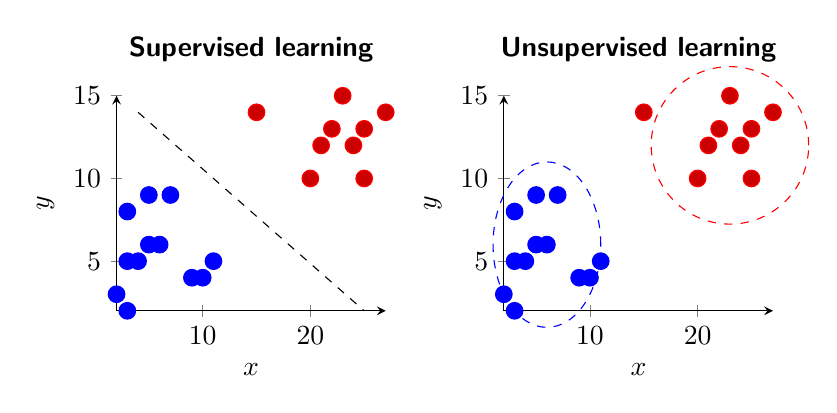
\begin{tikzpicture}
\begin{groupplot}[
group style={
  group size=2 by 1,
  horizontal sep=1.5cm
  },
axis lines = left,
xlabel = $x$,
ylabel = $y$,
width=5cm, % <-- set size of axes
clip mode=individual, % to avoid \draws being cut off
title style={yshift=1mm, font=\bfseries\sffamily}
]

\nextgroupplot[title=Supervised learning]
\addplot [blue, only marks, mark=*, mark size=3] table [%
x = x, 
y = y, 
col sep = comma]{
    x, y
    %cluster 1
    2, 3
    3, 5
    4, 5
    3, 8
    5, 9
    3, 2
    5, 6
    6, 6
    7, 9
    10, 4
    11, 5
    9, 4
    };
    
\addplot+[red, only marks, mark=*, mark size=3] table [%
x = x, 
y = y, 
col sep = comma]{
    x, y
    20, 10
    21, 12
    24, 12
    25, 13
    27, 14
    22, 13
    23, 15
    25, 10
    15, 14
 };
 
 % to be able to use axis coordinates with \draw directly you need
 % \pgfplotsset{compat=1.11} or a higher version
 % if that is not present, use (axis cs:4,14) instead of (4,14),
 % to specify that the values should be interpreted as axis coordinates
 \draw [dashed] (4,14) -- (25,2);
 

 
\nextgroupplot[title=Unsupervised learning]
\addplot [blue, only marks, mark=*, mark size=3] table [%
x = x, 
y = y, 
col sep = comma]{
    x, y
    %cluster 1
    2, 3
    3, 5
    4, 5
    3, 8
    5, 9
    3, 2
    5, 6
    6, 6
    7, 9
    10, 4
    11, 5
    9, 4
    };
    
\addplot+[red, only marks, mark=*, mark size=3] table [%
x = x, 
y = y, 
col sep = comma]{
    x, y
    20, 10
    21, 12
    24, 12
    25, 13
    27, 14
    22, 13
    23, 15
    25, 10
    15, 14
 };
 

 % save a coordinate for use later
 \coordinate (c2) at (23,12);
 
 % the blue circle is drawn inside the axis environment, and in axis coordinates
 % hence it becomes an ellipse
 \draw [blue, dashed] (6,6) circle[radius=5]; 

\end{groupplot}

% the red circle is drawn outside the axis, so actually looks like a circle,
% but the radius has no relation to the axis coordinates
\draw [red, dashed] (c2) circle[radius=1cm];


\end{tikzpicture}
\end{document}